\section{Tennis Ontology}\label{sec:result_t_ontology}
In this section, results from the crowd-sourced ontology validation in the domain of tennis are presented. A detailed discussion of the ontology used as a baseline for all calculations was done previously in \hyperref[sec:evaluation_datasets]{Section~\ref*{sec:evaluation_datasets}}.

The worker performance for this dataset was the highest among all evaluated ontologies. In fact, for the highest ranked method~\emph{(Metadata~based~Approach)} at least 2 out of 5 contributors correctly identified relevant concepts or declined unrelated ones. This corresponds to a precision of $0.896$ and recall of $0.976$, or combined F-Measure of $0.934$. A detailed comparison of all methods for this dataset is given in~\hyperref[table:bench_p_r_f_tennis]{Table~\ref*{table:bench_p_r_f_tennis}}. Interestingly, the \emph{Dictionary~based~Approach} performed worse than omitting concept descriptions at all. This, we noticed by the high discrepancy of precision. More precisely, $0.648$ with descriptions constructed from WordNik consultation~\emph{(Dictionary~based~Approach)} compared to $0.783$ without any context. 
\begingroup
\renewcommand{\arraystretch}{1.5}
\begin{table}
	\begin{tabularx}{\textwidth}{l c*{3}{Y}}
		\toprule
		Method & Precision & Recall & F-Measure \\
		\midrule
		 Metadata based Approach & 0.896 & 0.976 & 0.934 \\
		 Ontology based Approach & 0.874 & 0.939 & 0.905 \\ 
		 None & 0.783 & 0.933 & 0.851 \\
		 Dictionary based Approach & 0.648 & 0.980 & 0.780 \\
		\bottomrule
	\end{tabularx}
	\caption{Aggregated results on the Tennis Ontology~(ranked by F-Measure)}
	\label{table:bench_p_r_f_tennis}
\end{table}
\endgroup

\hyperref[fig:hist_agreement_tennis_all]{Figure~\ref*{fig:hist_agreement_tennis_all}} depicts the distribution of the agreement ratio among all validated concepts. To the contrary, by the \emph{Ontology~based~Approach}, crowd workers reached the most consensus, albeit being wrong in some cases. They declined 2 relevant concepts whereas for the \emph{Metadata~based~Approach} there were at least 2 of them who were correct for any concept. 
\begin{sidewaysfigure}
  	 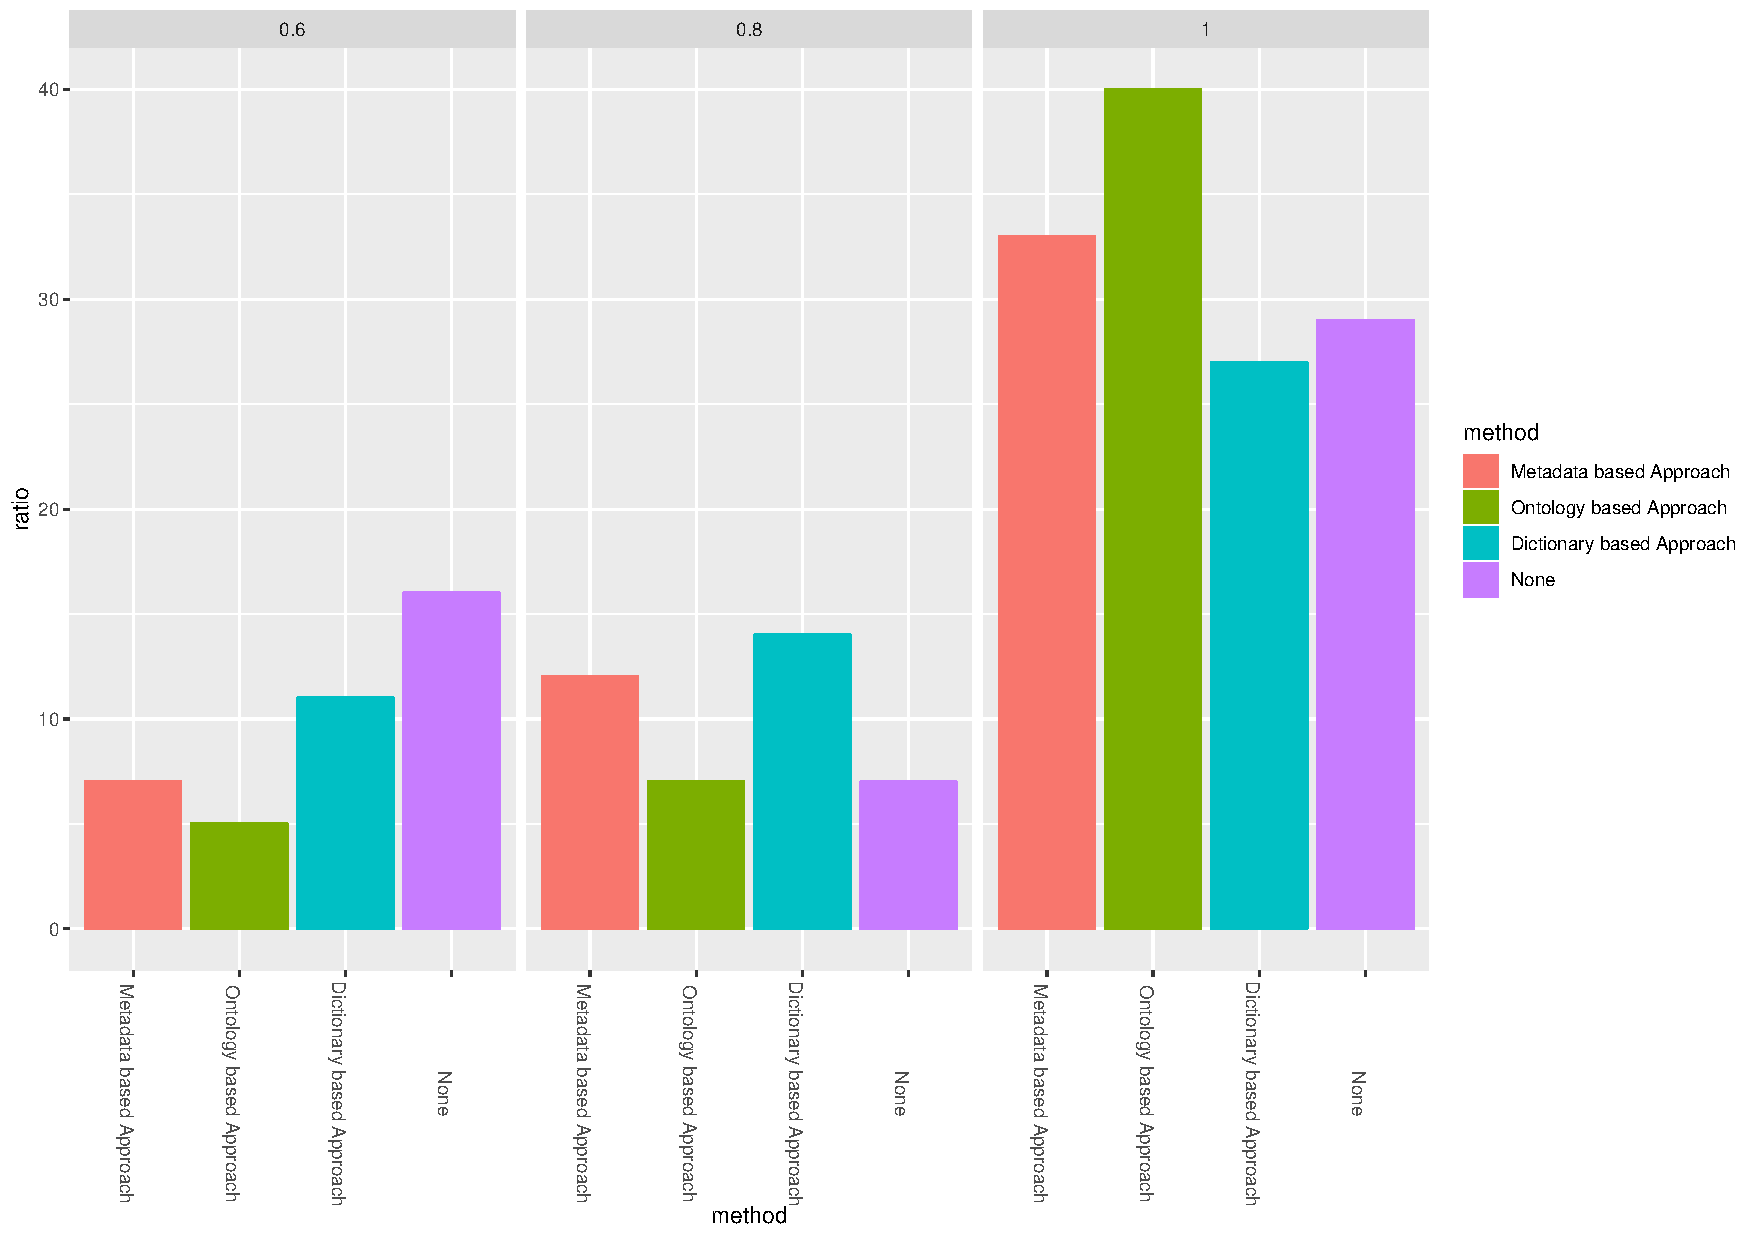
\includegraphics[width=\textwidth]{plots/tennis/hist_agreement_corrected}
  	 \caption{Histogram plots of the Inter-rater Agreement}\label{fig:hist_agreement_tennis_all}
\end{sidewaysfigure}

The observations from above were also reflected by the bar plots in~\hyperref[fig:hist_level_tennis_all]{Figure~\ref*{fig:hist_level_tennis_all}}. 
There were no judgments on level $-5$ and $-3$ for the \emph{Metadata~based~Approach}.
The summary statistics in~\hyperref[table:level_corr_incorr_tennis]{Table~\ref*{table:level_corr_incorr_tennis}} confirm that finding. Based on the agreement level and correct/incorrect judgement ratio, the rankings of each method were preserved. 
 
\begin{figure}
    \centering
    \begin{subfigure}[b]{0.4\textwidth}
        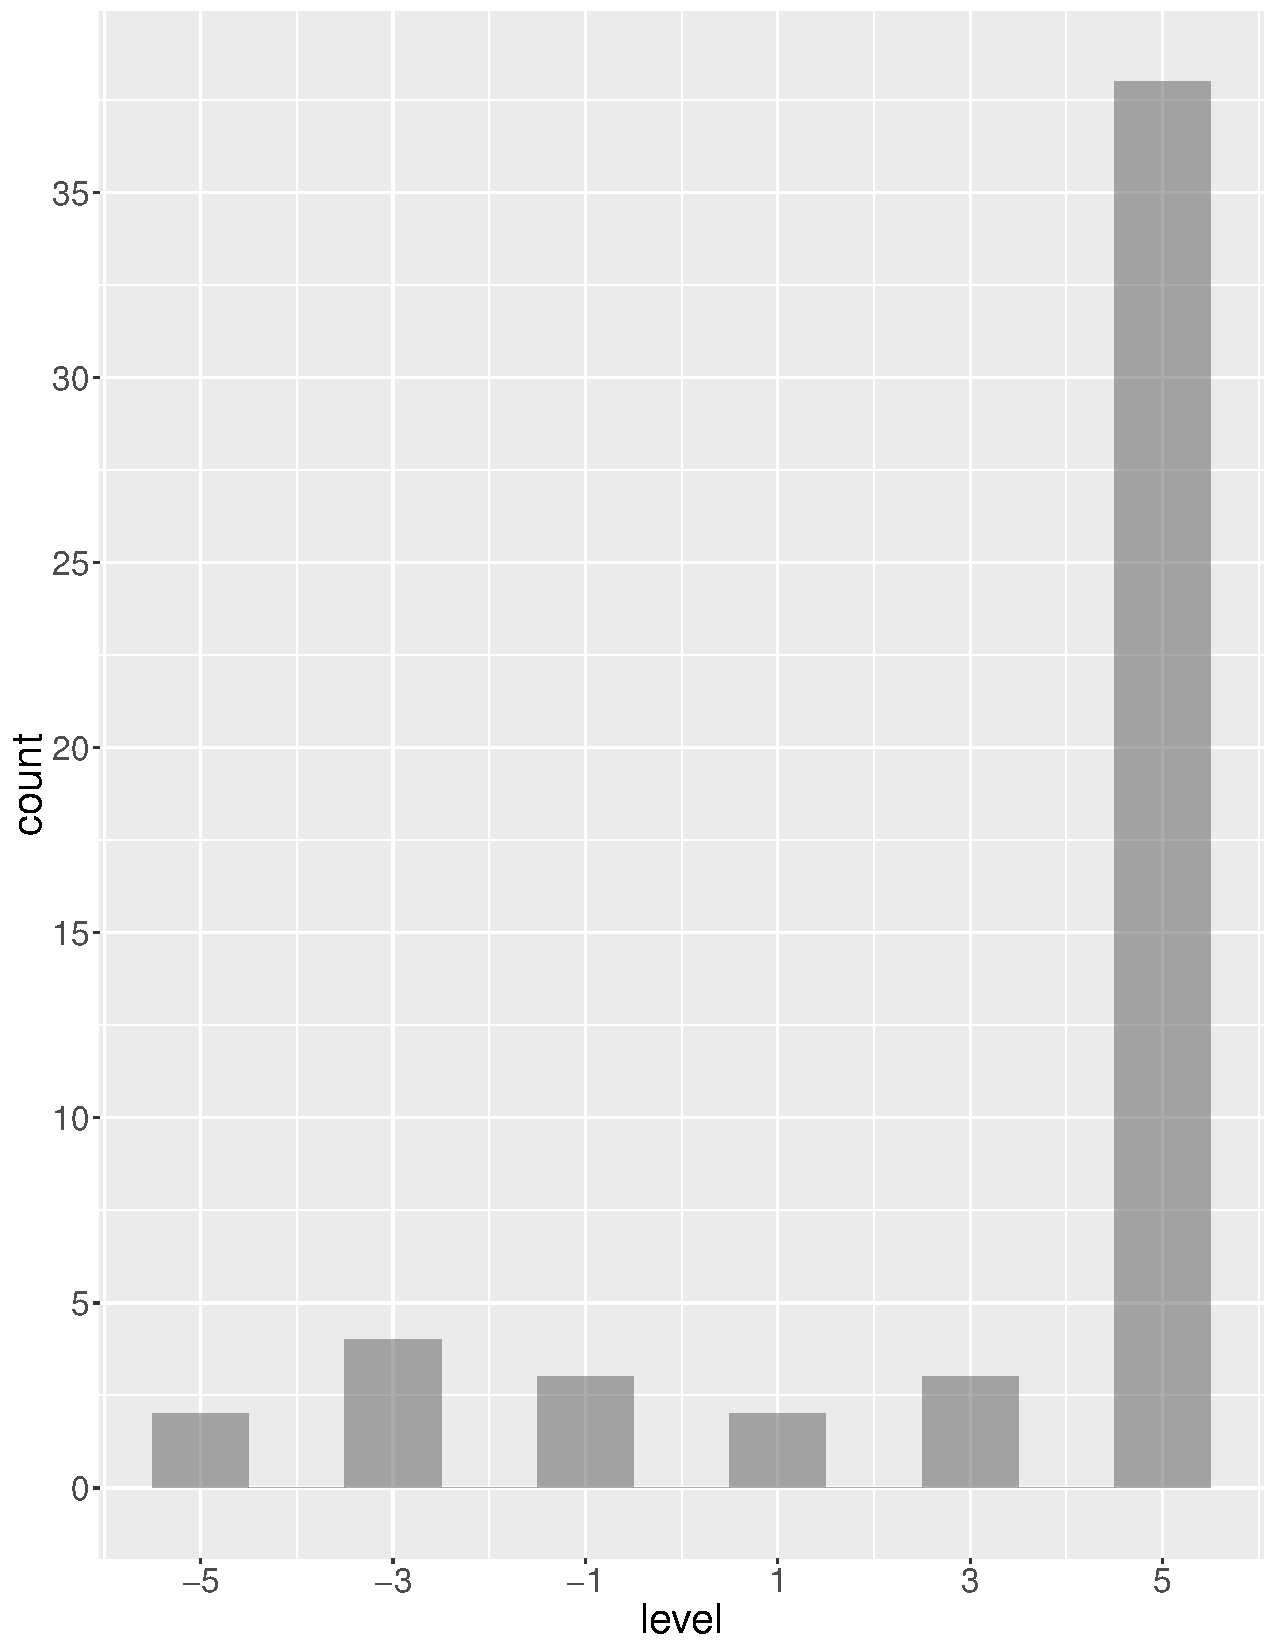
\includegraphics[width=\textwidth]{plots/tennis/hist_level_nn}
        \caption{Ontology based Approach}
        \label{fig:hist_level_tennis_nn}
    \end{subfigure}
    ~
    \begin{subfigure}[b]{0.4\textwidth}
        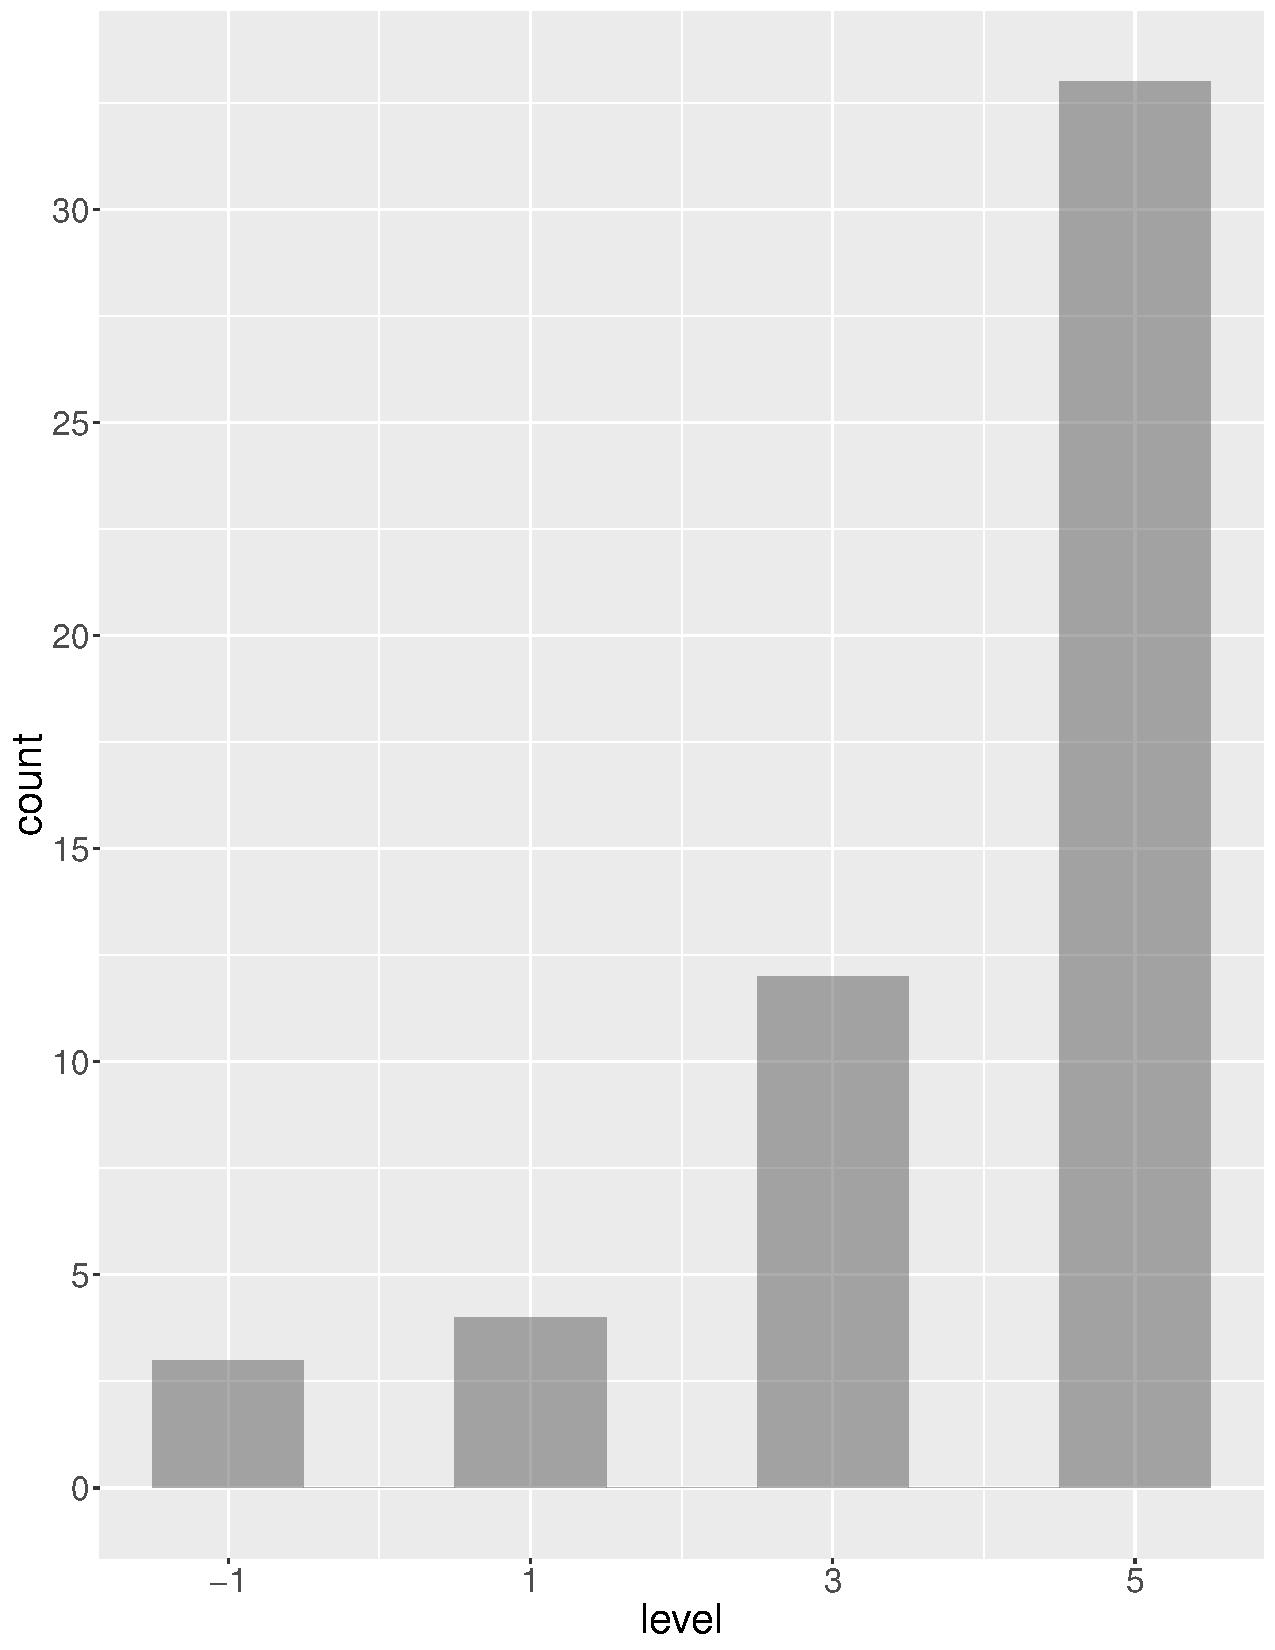
\includegraphics[width=\textwidth]{plots/tennis/hist_level_ec}
        \caption{Metadata based Approach}
        \label{fig:hist_level_tennis_ec}
    \end{subfigure}
    ~
    \begin{subfigure}[b]{0.4\textwidth}
        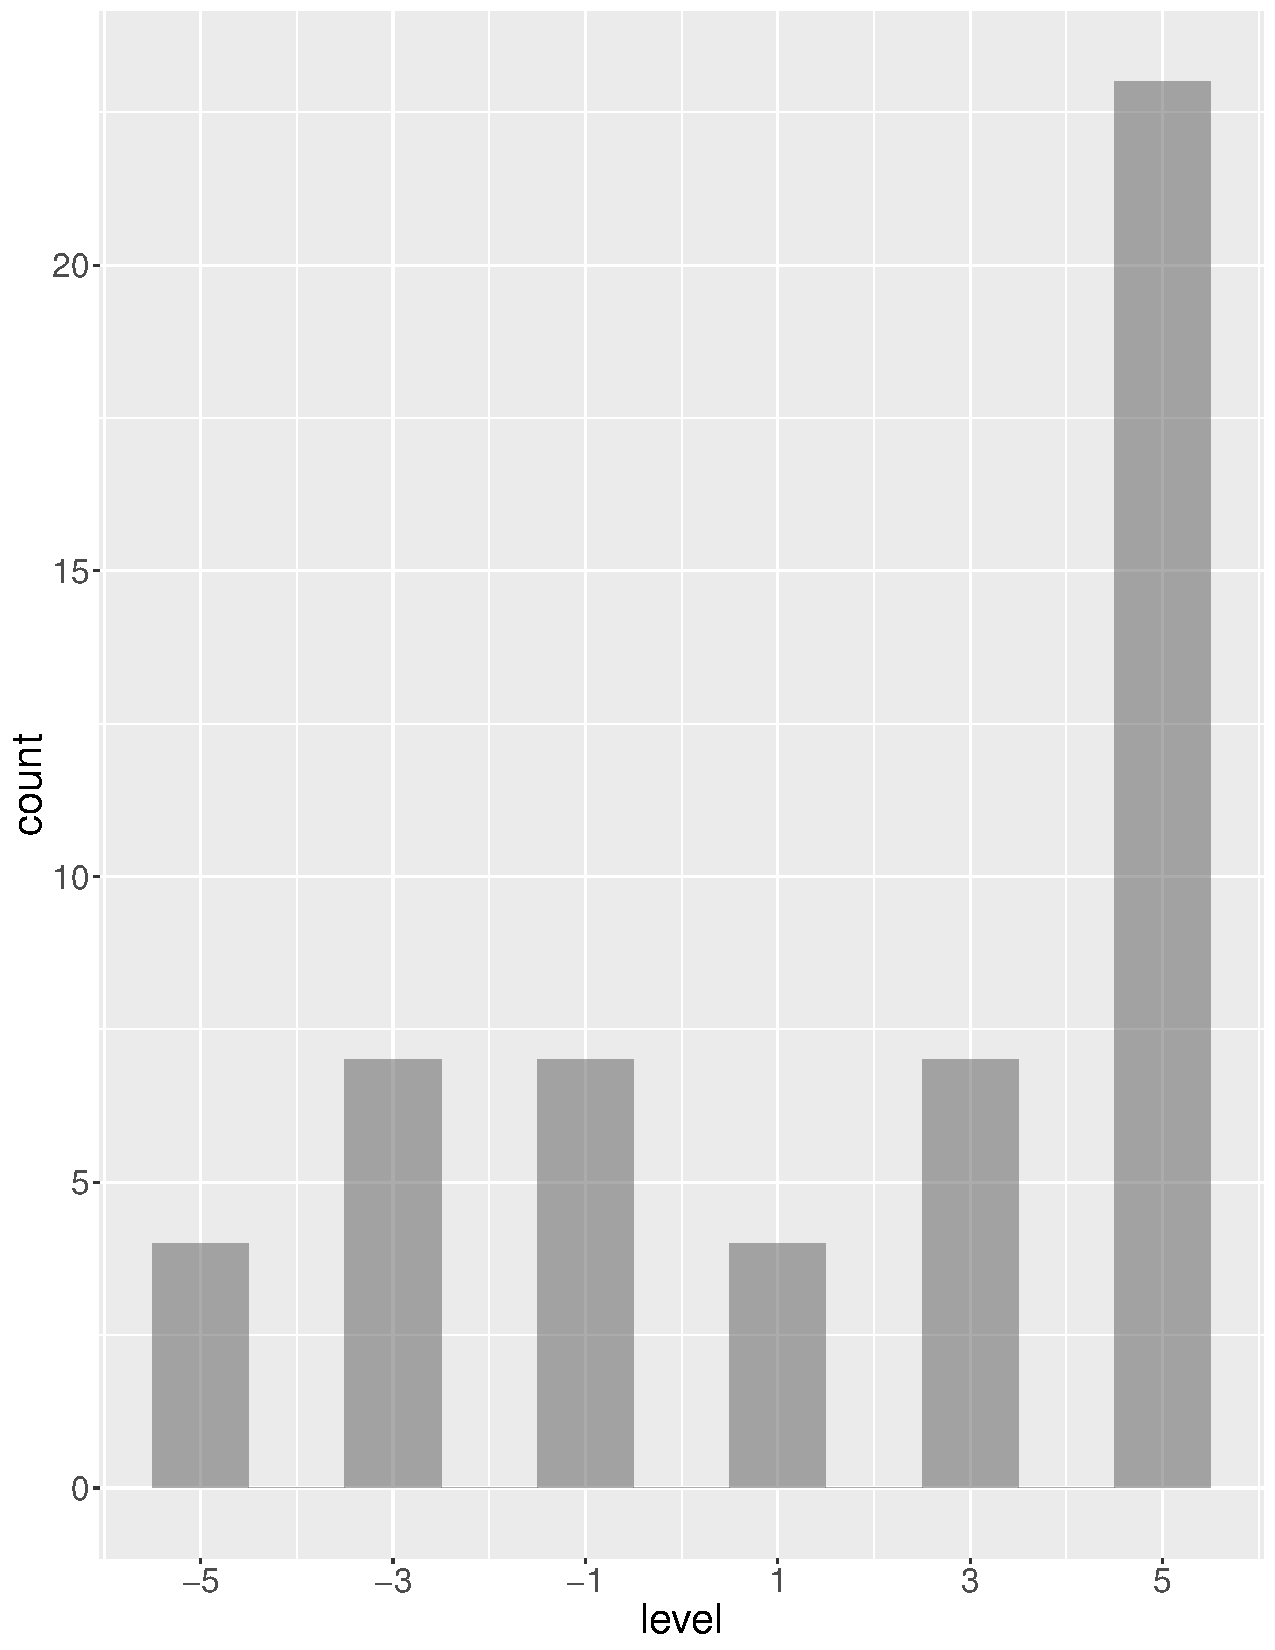
\includegraphics[width=\textwidth]{plots/tennis/hist_level_es}
        \caption{Dictionary based Approach}
        \label{fig:hist_level_tennis_es}
    \end{subfigure}
    ~
    \begin{subfigure}[b]{0.4\textwidth}
        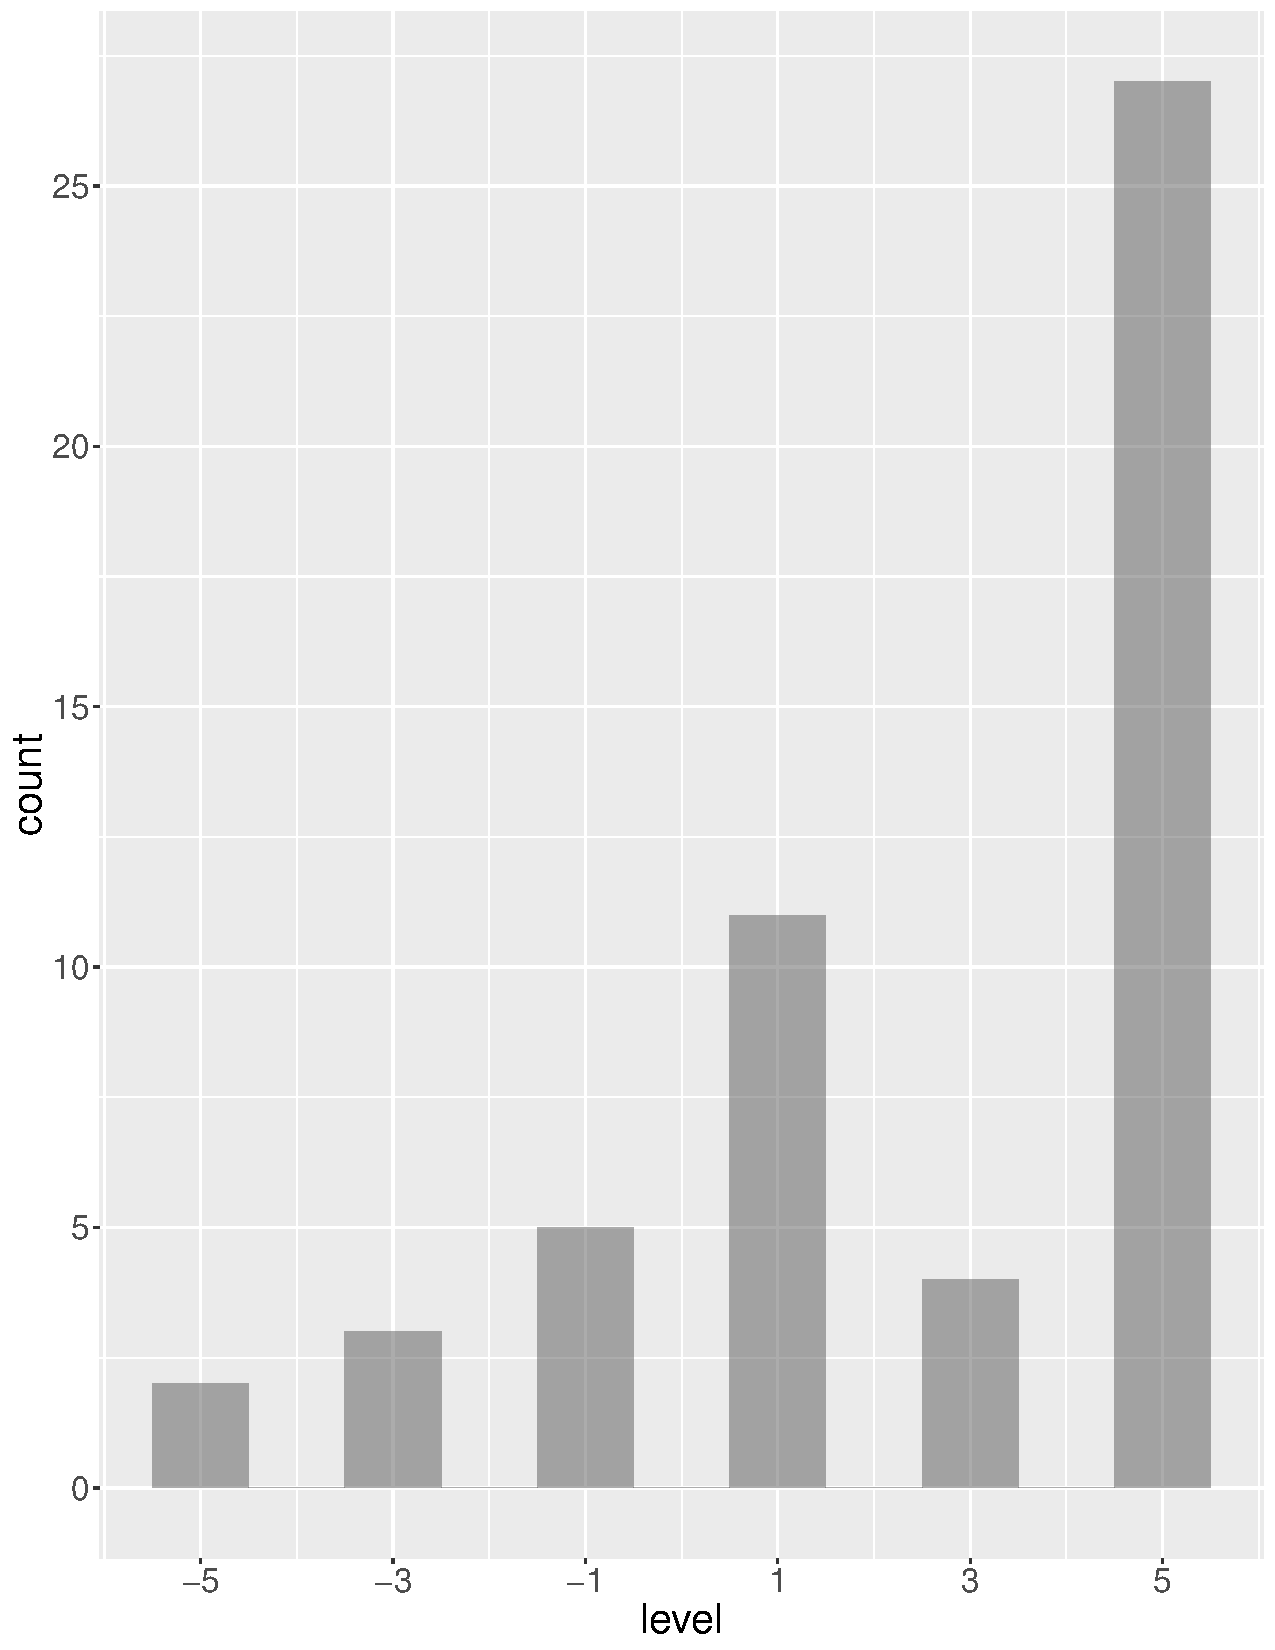
\includegraphics[width=\textwidth]{plots/tennis/hist_level_none}
        \caption{None}
        \label{fig:hist_level_tennis_none}
    \end{subfigure}
    \caption{Histogram plots of the correct/incorrect judgements. $\{$\emph{count}=number of judgements, \emph{level}=combined number of correct (positive scale) and incorrect (negative scale) judgements per concept$\}$ }
	\label{fig:hist_level_tennis_all}
\end{figure}


\begingroup
\renewcommand{\arraystretch}{1.5}
\begin{table}
	\begin{tabularx}{\textwidth}{l c*{4}{Y}}
		\toprule
		Method & mean & median & $1^{st}$ quartile & $3^{rd}$ quartile \\
		\midrule
		 Metadata based Approach & 3.89 & 5.00 & 3.00 & 5.00 \\
		 Ontology based Approach & 3.39 & 5.00 & 3.00 & 5.00 \\
		 None & 2.58 & 5.00 & 1.00 & 5.00 \\
		 Dictionary based Approach & 1.77 & 3.00 & -1.00 & 5.00 \\
		\bottomrule
	\end{tabularx}
	\caption{Summary statistics concerning agreement level on the Finance Ontology~(ranked by mean value)}
	\label{table:level_corr_incorr_tennis}
\end{table}
\endgroup